% This file is part of Combo Whist.
%
% Copyright 2014-2016 Joakim Nilsson
%
% This text is free software: you can redistribute it and/or modify
% it under the terms of the GNU General Public License as published by
% the Free Software Foundation, either version 3 of the License, or
% (at your option) any later version.
%
% This text is distributed in the hope that it will be useful,
% but WITHOUT ANY WARRANTY; without even the implied warranty of
% MERCHANTABILITY or FITNESS FOR A PARTICULAR PURPOSE.  See the
% GNU General Public License for more details.
%
% You should have received a copy of the GNU General Public License
% along with this text.  If not, see <http://www.gnu.org/licenses/>.
% License notice
% Packages

\usepackage[utf8]{inputenc}
\usepackage[protrusion=true]{microtype} % More readable layout
\usepackage{graphicx}                   % For \rotatebox
\usepackage{tabularx}                   % For the X column specifier
\usepackage[pass]{geometry}             % For changing margins
\usepackage[labelfont=bf]{caption}      % Captions boldface
\usepackage{siunitx}                    % Number alignment in tables
\usepackage{verbatim}
\usepackage{hyperref}

% Set-up reference style
\hypersetup{%
	pdfborderstyle={/S/U/W 1}
}

% Rotate text 90 degrees
\newcommand{\rotccw}[1] {%
	\rotatebox{90}{{#1}}
}

\newcommand{\standardBidItem}[6]{%
	\\ \hline
	\textit{#1} &
	#2 &
	#3 &
	#4 &
	#5 &
	#6
}

\newcommand{\specialBidItem}[4]{%
	\\ \hline
	\textit{#1} &
	#2 &
	\raggedright\textit{#3} &
	#4
}

\newcommand{\introPages}{%
	% Title
	\maketitle

	\vfill

	% Logo
	\begin{center}
		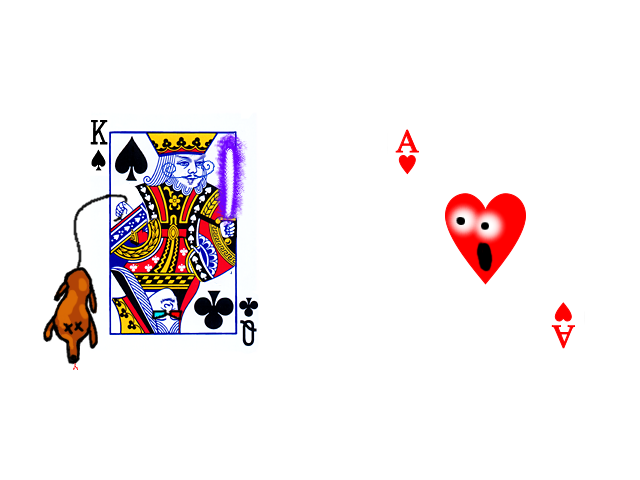
\includegraphics[width = \textwidth]{../logo.png}
	\end{center}

	\vfill

	% This file is part of Combo Whist.
%
% Copyright 2014-2016 Joakim Nilsson
%
% This text is free software: you can redistribute it and/or modify
% it under the terms of the GNU General Public License as published by
% the Free Software Foundation, either version 3 of the License, or
% (at your option) any later version.
%
% This text is distributed in the hope that it will be useful,
% but WITHOUT ANY WARRANTY; without even the implied warranty of
% MERCHANTABILITY or FITNESS FOR A PARTICULAR PURPOSE.  See the
% GNU General Public License for more details.
%
% You should have received a copy of the GNU General Public License
% along with this text.  If not, see <http://www.gnu.org/licenses/>.
% License notice

\begin{verbatim}
	Copyright 2007-2016 Joakim Nilsson

	This text is free software: you can redistribute it and/or modify
	it under the terms of the GNU General Public License as published by
	the Free Software Foundation, either version 3 of the License, or
	(at your option) any later version.

	This text is distributed in the hope that it will be useful,
	but WITHOUT ANY WARRANTY; without even the implied warranty of
	MERCHANTABILITY or FITNESS FOR A PARTICULAR PURPOSE.  See the
	GNU General Public License for more details.
\end{verbatim}
\verb|You should have received a copy of the GNU General Public License|\\
\verb|along with this text.  If not, see <|\url{http://www.gnu.org/licenses/}\verb|>.|


	\thispagestyle{empty}
	\pagebreak

	% Table of contents and list of tables without protrusion
	\microtypesetup{protrusion=false}
	\setcounter{tocdepth}{3}
	\tableofcontents
	\listoftables
	\microtypesetup{protrusion=true}
	\thispagestyle{empty}
	\pagebreak
}
